\section{Harvester}
\subsection{Harvester Architecture}

The harvester collects tweets from two major sources, one is tweet streaming and one is an online COVID-19 dataset. The streaming uses the python package tweepy to create a tweet listener, and the listener collects tweets under certain filtering conditions in real time. The second source makes the use of a online data website, IEEE, this website is updated daily with a worldwide summary of the IDs of COVID related tweets during that day.
\subsubsection{Data Collection Stage}
\paragraph{Streaming}

The streaming firstly create a listener to monitor the tweets posted in real time, a geo-location filter has been added to the listener so it will only collect tweets in Australia. The figure below illustrates an overview of this approach. 

\begin{figure}[h!]
\centering
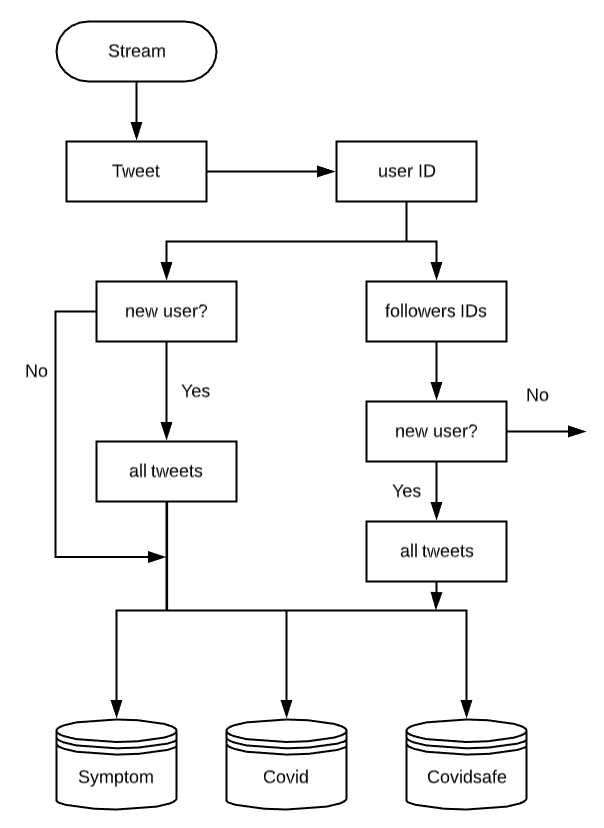
\includegraphics[scale=0.4]{city_analytics/report/images/stream.png}
\caption{streaming}
\label{fig:stream}
\end{figure}


For each tweet collected, the user who sent the tweet must be in Australia at the time the tweet was generated, a simple assumption is made here that the user is living in Australia, and thus, all tweets posted by that user can be also treated as in Australia even if some of tweets may not have exact geo-location information. 

Besides, another assumption made here is that most of the user's followers are also in Australia. And therefore, most of tweets posted by those followers can be treated as in Australia as well. However, the followers have a relatively larger probability that not in Australia, two addition filters have been added here to remove followers who have turned on the location service but have locations not in Australia and remove tweets that have locations not in Australia.

\paragraph{Online Dataset}

The online dataset contains a large list of tweet ids of the tweets related to COVID-19 around the world. The dataset has been used as a source to collect past tweets which cannot be collected by streaming. The flowchart below demonstrates the process of this method.
\begin{figure}[h!]
\centering
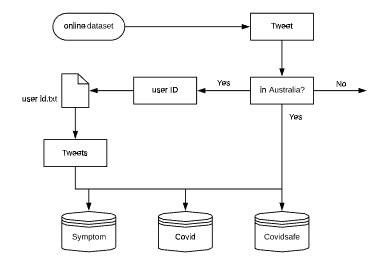
\includegraphics[scale=0.7]{city_analytics/report/images/online.png}
\caption{online dataset}
\label{fig:stream}
\end{figure}

Firstly, call Twitter API to retrieve all tweets using the tweet ids from the dataset, and pass the tweets into a filter to make sure only tweets in Australia will be collected. Secondly, same as before, the users of those collected tweets can be treated as Australian users and all tweets posted by those users can be treated as in Australia. In this methods, the followers of these users are not considered because these users have much larger probabilities that they are actually not in Australia because most of them does not turn on the location service.
\subsubsection{Deployment Stage}
When deploy on could, the streaming process has been slightly reduced to as following flowchart,

\begin{figure}[h!]
\centering
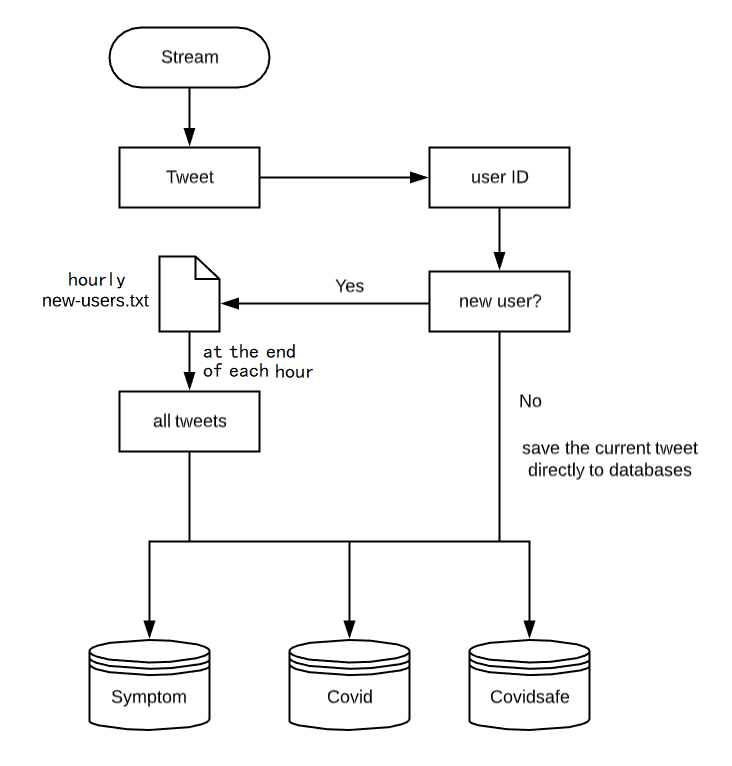
\includegraphics[scale=0.4]{city_analytics/report/images/deployment.png}
\caption{deploy}
\label{fig:stream}
\end{figure}

A new user file will be created daily to save the new users for that day. The harvester will start collecting tweets from those new users at a fixed time at the end of each day (23:57) and save them to couchDB. Followers are not considered when deploying on cloud because of the limitation of the numbers of accounts and the limits of Twitter API.

\subsection{Detail Implementation}

\subsubsection{Geo to SA4}
In this design, one of the requirements is to use tweet data in combination with Aurin. But this leads to problems as the location provided by tweets are in the form of exact geo coordinates instead of statistical area(SA) codes required by Aurin, and how to make use of the majority of tweets because only a very small portions of tweets have such coordinates. Therefore, it is necessary to figure out at least two different ways to covert the locations to SA codes.


For tweets with exact geo coordinates, the team firstly tried to use shape files provided by Australian Bureau of Statistics (ABS) to calculate the exact SA4 code for each coordinate. However, during implementation we noticed that there was a significant increasing in processing time for each tweet, the time suddenly jumped from less than 0.1 seconds to nearly 4 or 5 seconds after adding the converting function. The reason is the shape file provided by ABS has a very detailed boundary points of each area, therefore, finding the SA code for each coordinate becomes extremely slow due to the large amount to comparisons that need to be carried out. Therefore, we created a reduced version of the shapefile, the reduced shape file contains much less boundary points than the original one and the file size drops from 40MB to 1MB. Upon test, we noticed that in most of cases the reduced shape file can get the same SA code as the original file, only very few coordinates have wrong results but all within an acceptable range, for instance, an coordinate actually belongs to SA4 206 but the result is SA4 207.

For tweets without exact geo coordinates but have location names, the team created a dictionary file to match each suburb name with SA4 codes. As a result, this matching has a less accuracy than using the geo coordinate, thus, a new entity has been add to each tweet to show the source of the SA code, for instance, the new entity value is 'geo' if there is a coordinate, otherwise it will show 'name' which means the SA4 is from matching with the dictionary, and 'none' for tweets with neither coordinates nor names.

\subsubsection{Timestamp}
In future MapReduce stage, to avoid repeated analysis of previous data, a timestamp is add to each tweet to show the time that the tweet is been collected. The new data coming into the database will always has a larger timestamp than all tweets that already in the database. By doing this, every time when run MapReduce in future the script will only process the tweets have timestamp larger than the largest timestamp of the previous record.
\subsubsection{Duplication Control}
The fundamental source for this harvester is a list of unique user IDs. When a tweet comes in, firstly check whether the user ID is already in our users database or not. The harvester will only write the user id into a new user file and wait for further process only in the case that the user id does not exist in our users database, otherwise the harvester will only store the current tweet into couchDB with no further action because all of the previous tweets of that user have already been processed before.

A second layer to prevent duplication is the key used store tweets in couchDB. Every tweet has a unique ID, no two different tweets have the same ID, and this ID for new tweets keeps growing as people keep tweeting. Thus, when designing the couchDB databases, including the tweet ID as one part of the partition key is able to efficiently prevent duplicated tweets from storing all of them into the databases.
\subsubsection{Error Handling}
\paragraph{RateLimitError}In the harvester design, the main issue need to be aware of is Twitter has set up strict rate limits for developer accounts. If the limits cannot be handled properly, the account might be banned as a result of keeping hitting the limit.
The package tweepy allows users to set up a parameter and wait for 15 minutes once the API reaches the limit. However, by doing this the efficiency of the harvester will be greatly reduced because most of time the harvester is waiting instead of running. Thus, we used multiple accounts to keep it running.

The API used in this harvester is user timeline which returns a list of tweets of a specific user since a specific date. By testing, one account reaches its limit after running for around 5 to 7 minutes. Thus theoretically, three accounts is enough to keep the harvester running. But in practice, we use four accounts for one harvester in order to ensure a certain tolerance. These accounts are running in a rotating cycle, once a account reaches its limit, change to another key and continue running.

\paragraph{ResourceConflict}
When collecting data, more or less we inevitably get some duplicate tweets. Repeatedly storing same data into couchDB will raise an error ResourceConflict. Since tweet ID is unique, there is no need to store two tweets with same ID again, the harvester will ignore the tweet when raising a ResourceConflict error.

\subsubsection{Sentiment Analysis}
Sentiment reflects the user's attitude when sending the tweet. Sentiment analysis is achieved by analysing the content of tweets using a python library Textblob. For each tweet, the result can be either positive, neutral or negative.

\subsubsection{Simplify Tweet Structure}
Tweets from Twitter API have a complicated structure with lots of information. However, not all of the information is useful for this project. Cutting off some useless entities can not only reduce the space required to store those tweets, but most importantly can also reduce a significant amount of time used to query the tweets. Therefore, we only keep the most important information for us and the simplified tweet structure is illustrated as below:

\begin{figure}[h!]
\centering
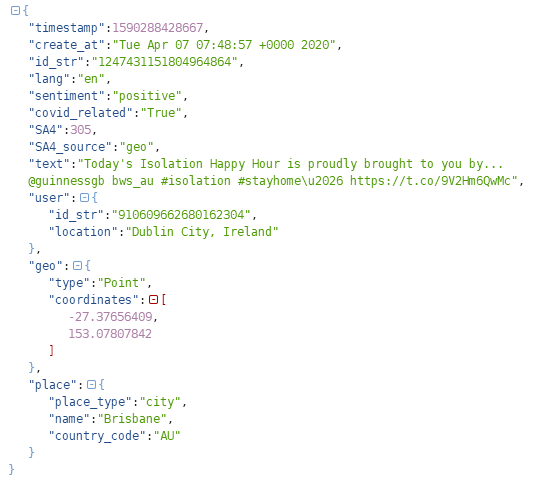
\includegraphics[scale=0.7]{city_analytics/report/images/simplifiedtweet.png}
\caption{simplified tweet}
\label{fig:stream}
\end{figure}


\subsection{Scalability}

Scalability is a critical part of a cloud-based design, a harvester should have the ability to deal with any given topic when deploying more instances and should also be able to maximize the use of given resources to achieve best efficiency.

Therefore, in this project, harvester is parameterized so it is able to deal with any need of getting tweets for a given topic. The input for the harvester is a customized Json as shown below,

\begin{figure}[h!]
\centering
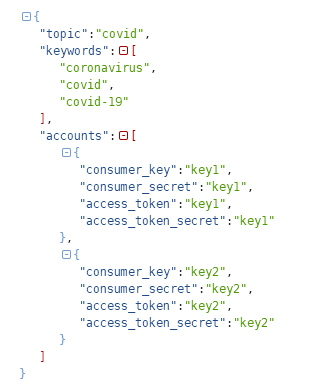
\includegraphics[scale=0.8]{city_analytics/report/images/harvester_input.png}
\caption{input parameter}
\label{fig:input parameter}
\end{figure}


The harvester takes topic, keywords and accounts as input. For any given topic, the harvester creates multiple threads to harvest tweets using the keywords provided. The number of threads depends on the number of twitter developer accounts provided. By testing, four accounts are enough to guarantee a thread to keep running without reaching its limit. Therefore, more keys means the harvester can create more threads so the collecting time will be reduced. Keys for threads are not uniformly distributed, one rule used here is try to give each thread 4 keys before create another thread, for instance, 4 accounts 1 thread, 6 accounts 2 thread (one with 4 accounts and one with 2 accounts), 10 accounts 3 threads (two threads with 4 accounts and one with 2 accounts) etc. Accordingly, load for each thread are not uniformly distributed and is proportional to the number of keys each thread are allocated. Therefore, thread with less keys will be allocated with less loads to make sure all threads will finish their tasks in a relative close point in time. For the thread with less than 4 keys, the thread may need to sleep for a specific amount of time to prevent it from keep hitting the limit.


\subsection{Limitation}
\subsubsection{Rate limit of API}

The harvester efficiency is mainly restricted by the API limit. Fewer keys in rotation means more likely to reach the limits. In contrast, more keys means we can divide the IDs into several portions and run them separately with multi threads. 

\subsubsection{Few users turn on location service}
As people are paying more attention to their privacy, only a few users would like to turn on the location service when using an application, which makes it is difficult to collect enough data with exact coordinates. We found that only 1\% of collected tweets have exact geo coordinates which may result in decreased accuracy of the analysis results.
